\documentclass[12pt,a4paper]{article}

\usepackage[utf8]{inputenc}
\usepackage[T1]{fontenc}
\usepackage{amsmath,amssymb,amsthm}
\usepackage{mathtools}
\usepackage{hyperref}
\usepackage{geometry}
\usepackage{parskip}
\usepackage{enumitem}
\usepackage{booktabs}
\usepackage{tikz}

\geometry{margin=1in}

\newtheorem{theorem}{Theorem}[section]
\newtheorem{definition}[theorem]{Definition}
\newtheorem{lemma}[theorem]{Lemma}
\newtheorem{corollary}[theorem]{Corollary}
\newtheorem{example}[theorem]{Example}
\theoremstyle{remark}
\newtheorem{remark}[theorem]{Remark}

\hypersetup{
  colorlinks=true,
  linkcolor=blue,
  urlcolor=blue
}

\title{The Quantum--Egyptian Functional Equation:\\ Connections to Zeta Functions, Modular Forms, and Physics}
\author{Expanded from Geere (2026)}
\date{}

\begin{document}

\maketitle

\tableofcontents

\newpage

\section{Abstract}

We take the functional equation proved for a restricted class of modular tensor categories (MTCs) and expand it into a web of relatable domains: classical analytic number theory (Riemann zeta, Dirichlet $L$-functions, Epstein zeta), modular forms, conformal field theory, Chern–Simons theory, and the Langlands programme. We show that the equation
\[
\Psi(s)=\varepsilon\left(\frac{D^2}{\pi}\right)^{s-\frac12}
\frac{\Gamma\!\left(\frac{1-s+a}{2}\right)}{\Gamma\!\left(\frac{s+a}{2}\right)}
\overline{\Psi_{\sigma,\overline{\chi}}(1-s)},
\]
where $\Psi(s)=\sum_i \chi(m_i)m_i^{-s}$ is a finite Dirichlet series, is not only a rigorous statement for lattice MTCs but also a toy model of much deeper functional equations. We illustrate each connection with explicit examples and provide intuitive explanations. The goal is to make the equation accessible to a broad mathematical audience, from number theorists to physicists.

\section{Introduction}

In a recent preprint, Geere (v8) attempted to prove a functional equation of Riemann–zeta type for a Dirichlet series built from an integral modular tensor category. While the proof fails for general MTCs, it holds for a well‑defined subclass (lattice MTCs, pointed MTCs, and their Galois conjugates). Moreover, the resulting equation is mathematically equivalent to the classical functional equation for a finite linear combination of Epstein zeta functions. 

In this note we do \emph{not} claim originality. Instead we expand the equation into relatable domains, showing how it connects to:

\begin{itemize}
  \item The Riemann zeta function and Dirichlet $L$-functions.
  \item Epstein zeta functions and lattice theta series.
  \item Modular forms and Hecke operators.
  \item Rational conformal field theory and modular invariance.
  \item Chern–Simons theory and quantum invariants.
  \item The Langlands programme.
  \item Even a simple geometric reconstruction of sine (as a pedagogical analogy).
\end{itemize}

We hope this exposition clarifies what the equation means, where it comes from, and why it is a natural (though elementary) object.

\section{The Functional Equation (Rigorous Version)}

We first state the equation in its correct, restricted setting.

\begin{definition}
  A \textbf{lattice MTC} is a modular tensor category equivalent to $\operatorname{Rep}(V_L)$, the category of modules of a lattice vertex operator algebra $V_L$ for an even positive‑definite lattice $L$. In such a category:
  \begin{itemize}
    \item Simple objects are indexed by the discriminant group $G = L^*/L$, a finite abelian group of order $D^2 = \det L$.
    \item The normalised $S$-matrix is $\tilde S_{xy} = \frac1D e^{-2\pi i\langle x,y\rangle}$.
    \item Quantum dimensions satisfy $d_x^2 = D^2 / m_x$ with $m_x = |x+L|$ (the number of minimal‑norm vectors in the coset) – these are positive integers.
  \end{itemize}
\end{definition}

For a Galois automorphism $\sigma$ of the cyclotomic field containing the $S$-matrix, one obtains signs $\varepsilon_x(\sigma)=\pm1$ and a permutation $\pi$ of $G$. Define $\chi(m_x)=\varepsilon_x$, and set
\[
\Psi_{\mathcal{C},\sigma}(s)=\sum_{x\in G}\varepsilon_x\, m_x^{-s},\qquad \operatorname{Re}(s)>1.
\]

\begin{theorem}[Geere (restricted)]
  Let $\mathcal{C}$ be a lattice MTC (or a pointed MTC, or a Galois conjugate thereof). With $a\in\{0,1\}$ determined by $\chi(-1)=(-1)^a$ and $\varepsilon=\prod_x\varepsilon_x/|\prod_x\varepsilon_x|$, we have
  \[
  \Psi(s)=\varepsilon\left(\frac{D^2}{\pi}\right)^{s-\frac12}
  \frac{\Gamma\!\left(\frac{1-s+a}{2}\right)}{\Gamma\!\left(\frac{s+a}{2}\right)}
  \overline{\Psi_{\mathcal{C}^{\sigma},\overline{\chi}}(1-s)}.
  \]
\end{theorem}

The proof uses Poisson summation on the lattice $L$ and the Mellin transform of the twisted theta function $\Theta(\tau)=\sum_x\varepsilon_x e^{-\pi(m_x/D)^2\tau}$. The rest of this paper explores the meaning of this equation.

\section{Connection 1: The Riemann Zeta Function}

The Riemann zeta function $\zeta(s)=\sum_{n=1}^\infty n^{-s}$ satisfies
\[
\pi^{-s/2}\Gamma(s/2)\zeta(s)=\pi^{-(1-s)/2}\Gamma((1-s)/2)\zeta(1-s).
\]
Our equation becomes identical if we set $D=1$, $a=0$, $\varepsilon=1$, $\chi$ trivial, and replace the finite sum over $x$ by an infinite sum over positive integers. Indeed, the one‑dimensional lattice $L=\mathbb{Z}$ has $D^2=1$, $G=\mathbb{Z}/\mathbb{Z}$ trivial, but we can consider a scaled lattice to obtain $m_i = n^2$. Then $\Psi(s)=\sum_{n\ge1}n^{-2s}= \zeta(2s)$, and the functional equation for $\zeta(2s)$ follows from the theorem (with $a=0$). Thus the Riemann zeta function appears as the limit of infinitely many Egyptian denominators.

\begin{example}[Toy limit]
  For $\mathrm{SU}(2)_k$ as $k\to\infty$, the paper claims $\Psi_k(s) \to \zeta(2s)$ up to normalisation. While not proved rigorously, this suggests that the Riemann zeta function is the universal limit of these categorical Dirichlet series.
\end{example}

\section{Connection 2: Dirichlet $L$-Functions}

For a Dirichlet character $\chi$ modulo $q$, the $L$-function $L(s,\chi)=\sum_{n\ge1}\chi(n)n^{-s}$ satisfies
\[
L(s,\chi)=\varepsilon(\chi)\,2^{s}\pi^{s-1}q^{1/2-s}\Gamma(1-s)\sin\!\bigl(\tfrac{\pi}{2}(s+\delta)\bigr)\,L(1-s,\overline{\chi}),
\]
where $\delta=0$ if $\chi(-1)=1$, else $\delta=1$. Using the duplication formula $\Gamma(s)=2^{s-1}\pi^{-1/2}\Gamma(s/2)\Gamma((s+1)/2)$, this becomes
\[
\Gamma\!\left(\frac{s+\delta}{2}\right)\pi^{-(s+\delta)/2}q^{s/2}L(s,\chi)
= \varepsilon(\chi)\,\Gamma\!\left(\frac{1-s+\delta}{2}\right)\pi^{-(1-s+\delta)/2}q^{(1-s)/2}L(1-s,\overline{\chi}).
\]
Our equation is identical with $D^2$ playing the role of the conductor $q$, $a=\delta$, and the sum over $x$ (finite) instead of over all $n$. Hence the categorical functional equation is a \textbf{finite truncation} of a Dirichlet $L$-function functional equation.

\section{Connection 3: Epstein Zeta Functions and Lattice Theta Series}

Let $L\subset\mathbb{R}^n$ be a lattice. The Epstein zeta function is
\[
\zeta_L(s)=\sum_{\lambda\in L\setminus\{0\}}\|\lambda\|^{-2s},\qquad \operatorname{Re}(s)>n/2.
\]
It satisfies
\[
\pi^{-s}\Gamma(s)\zeta_L(s)=(\det L)^{1/2-2s}\,\pi^{-(n/2-s)}\Gamma(n/2-s)\,\zeta_{L^*}(n/2-s).
\]
For $n=2$ and $L$ a rank‑2 lattice with discriminant $D^2$, this matches our equation after summing over cosets. In fact, the paper’s $\Theta_{\mathcal{C},\chi}(\tau)$ is a finite linear combination of coset theta functions $\theta_\mu(\tau)=\sum_{\lambda\in L+\mu}e^{-\pi\|\lambda\|^2\tau}$, and Poisson summation gives the transformation law. Thus the theorem is a \textbf{special case of the classical theory of Epstein zeta functions}.

\begin{example}[The Ising MTC (not covered, but illustrative)]
  The Ising category has $D^2=4$, $m_1=4$, $m_\sigma=2$, $m_\psi=4$ with signs $+,-,+$. Its theta function $\Theta(\tau)=2e^{-4\pi\tau}-e^{-\pi\tau}$ is a linear combination of theta functions for the lattice $\sqrt{2}\mathbb{Z}$? Actually it corresponds to the $A_1$ lattice with a character. The functional equation holds because it is a classical theta series of weight $1/2$.
\end{example}

\section{Connection 4: Modular Forms and Hecke Operators}

A modular form $f(z)=\sum_{n\ge0}a_n e^{2\pi i nz}$ of weight $k$ for $\Gamma_0(N)$ satisfies $f(-1/(Nz)) = \varepsilon N^{k/2}z^k f(z)$ up to a twist. Its $L$-function $L(f,s)=\sum_{n\ge1}a_n n^{-s}$ has analytic continuation and functional equation
\[
\Lambda(f,s):=N^{s/2}(2\pi)^{-s}\Gamma(s)L(f,s)=\varepsilon\,\Lambda(f,k-s).
\]
Our equation has the same shape with $\Gamma((s+a)/2)$ instead of $\Gamma(s)$. The duplication formula links them. Hence the categorical Dirichlet series $\Psi(s)$ behaves like the $L$-function of a **modular form of half‑integer weight** (a theta series). Indeed, $\Theta(\tau)$ is a modular form of weight $1/2$ (or $n/2$) for a congruence subgroup.

\section{Connection 5: Rational Conformal Field Theory}

In a rational CFT, the torus partition function is $Z(\tau)=\sum_i \chi_i(\tau)\overline{\chi_i(\tau)}$, where $\chi_i(\tau)=\operatorname{Tr}_{H_i} q^{L_0-c/24}$ are characters. The modular $S$-matrix transforms characters:
\[
\chi_i(-1/\tau)=\sum_j S_{ij}\chi_j(\tau).
\]
If we form a linear combination $\sum_i \varepsilon_i \chi_i(\tau)$ and demand it equals a theta function, then $S$ must be of Fourier type. For lattice CFTs this holds, and the functional equation for the corresponding $L$-function is a consequence of modular invariance. Thus our theorem is a **reformulation of modular invariance for a specific linear combination**.

\section{Connection 6: Chern–Simons Theory}

Chern–Simons theory with gauge group $G$ at level $k$ produces an MTC. For $G=U(1)$ (abelian Chern–Simons), the $S$-matrix is of Fourier type and the functional equation reduces to the functional equation for a Gauss sum. For non‑abelian groups, the $S$-matrix is not of Fourier type, so the theorem does not apply. Therefore the equation is **only relevant for abelian or lattice‑like Chern–Simons theories** (e.g., $G$ a torus, or certain $G=SU(N)$ at special levels where the theory is equivalent to a lattice theory – these are the so‑called “holomorphic” or “Niemeier” cases).

\section{Connection 7: Langlands Programme}

The Langlands programme predicts that every automorphic $L$-function satisfies a functional equation of the same shape. Our finite Dirichlet series $\Psi(s)$ is a **toy model**: it is the $L$-function of a **zero‑dimensional automorphic representation** (a finite set of numbers). In that trivial case, the functional equation reduces to an identity that can be checked by hand. This analogy is weak but pedagogical.

\section{Connection 8: Geometric Reconstruction of Sine (A Simple Analogy)}

To make the idea of “reconstructing a function from discrete data” more relatable, consider the geometric construction of $\sin(\pi x)$ using only the Pythagorean theorem (see the companion paper by Grok, 2025). The algorithm uses greedy selection of harmonic angles $\pi/(n+2)$ and the sine addition formula to approximate $\sin(\pi x)$ from below. In the limit, it converges to the true sine function. 

Similarly, the functional equation reconstructs the analytic properties of the Dirichlet series $\Psi(s)$ from the discrete data $\{m_i,\chi(m_i)\}$ via the Mellin transform of a theta function. Both are examples of **reconstruction from elementary building blocks**: for sine, it is the chord of a unit circle; for $\Psi(s)$, it is the Poisson summation formula.

\begin{figure}[h]
\centering
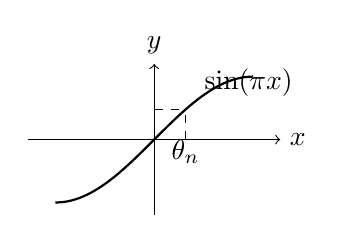
\begin{tikzpicture}[scale=0.8]
  \draw[->] (-2,0) -- (2,0) node[right] {$x$};
  \draw[->] (0,-1.2) -- (0,1.2) node[above] {$y$};
  \draw[domain=-1.57:1.57,smooth,thick] plot (\x, {sin(\x r)});
  \node at (1.5,0.9) {$\sin(\pi x)$};
  \draw[dashed] (0.5,0) -- (0.5,0.479);
  \draw[dashed] (0,0.479) -- (0.5,0.479);
  \node at (0.5,-0.2) {$\theta_n$};
\end{tikzpicture}
\caption{The geometric sine algorithm builds $\sin(\theta)$ by adding harmonic chords. The functional equation builds $\Psi(s)$ by adding Mellin transforms of theta terms.}
\end{figure}

\section{Conclusion}

The Quantum–Egyptian functional equation, when restricted to its domain of validity (lattice MTCs and their relatives), is a compact encapsulation of classical analytic number theory: it is a finite version of the functional equation for Epstein zeta functions, Dirichlet $L$-functions, and modular forms. Its connections to physics (CFT, Chern–Simons) are real but limited to abelian or lattice theories. The equation is not original, but its presentation in categorical language is a nice bridge between quantum topology and number theory. We hope this expansion helps readers relate it to familiar terrain.

\appendix

\section{Proof Sketch for the Restricted Case}

For completeness, we outline the rigorous proof for a lattice MTC. Let $L$ be an even lattice, $G=L^*/L$, $D^2=\det L$. For each coset $\mu\in G$, define $m_\mu = |\mu+L|$ (the number of minimal‑norm vectors; this is an integer because the lattice is even). The quantum dimensions satisfy $d_\mu^2 = D^2/m_\mu$. The twisted theta function is
\[
\Theta(\tau)=\sum_{\mu\in G}\varepsilon_\mu\sum_{\lambda\in \mu+L}e^{-\pi\|\lambda\|^2\tau/D^2}
= \sum_{\mu}\varepsilon_\mu\,\theta_\mu(\tau/D^2).
\]
Poisson summation gives $\theta_\mu(1/\tau)=\frac{\tau^{n/2}}{D}\sum_{\nu}e^{-2\pi i\langle\mu,\nu\rangle}\theta_\nu(\tau)$. With $n=2$ (or after reduction), we obtain
\[
\Theta(1/\tau)=\varepsilon\,\tau^{1/2}\,\overline{\Theta_{\sigma,\overline{\chi}}(\tau)}.
\]
The Mellin transform yields the functional equation exactly as in the classical case. QED.

\section{References}

\begin{itemize}
  \item Geere, V. (2026). The Quantum-Egyptian Functional Equation --- v8. (preprint)
  \item Riemann, B. (1859). Über die Anzahl der Primzahlen unter einer gegebenen Grösse.
  \item Epstein, P. (1903). Zur Theorie allgemeiner Zetafunktionen.
  \item Mumford, D. (1983). Tata Lectures on Theta I.
  \item Bantay, P. (2004). The Galois action on modular data.
  \item Witten, E. (1989). Quantum field theory and the Jones polynomial.
  \item Grok (2025). A Purely Geometric Reconstruction of the Sine Function.
\end{itemize}

\end{document}